% ============================================================
%  Meridian Capital - Asset Management Challenge 2026
%  Round 1: Strategic Asset Allocation
%  Compile with XeLaTeX
% ============================================================
\documentclass[10pt,a4paper]{article}

\usepackage{fontspec}
\defaultfontfeatures{Ligatures=TeX}
\setmainfont{DMSans}[
  Path=fonts/, Extension=.ttf,
  UprightFont=*-Regular, BoldFont=*-Bold,
  ItalicFont=*-Italic, BoldItalicFont=*-BoldItalic]
\setsansfont{DMSans}[
  Path=fonts/, Extension=.ttf,
  UprightFont=*-Regular, BoldFont=*-Bold,
  ItalicFont=*-Italic, BoldItalicFont=*-BoldItalic]
\renewcommand{\familydefault}{\sfdefault}
\usepackage{microtype}
\usepackage[a4paper,top=2.8cm,bottom=2.6cm,left=2.5cm,right=2.5cm,headheight=22pt]{geometry}
\addtolength{\topmargin}{-8pt}
\usepackage{amsmath,amssymb}
\usepackage{graphicx}
\graphicspath{{figures/}}
\usepackage{xcolor}
\usepackage{booktabs,array,tabularx,colortbl}
\usepackage{enumitem}
\usepackage{float}
\usepackage{needspace,etoolbox}
\pretocmd{\section}{\Needspace{12\baselineskip}}{}{}
\usepackage{titlesec}
\usepackage{fancyhdr}
\usepackage{caption}
\usepackage{listings}
\usepackage[most]{tcolorbox}
\usepackage{tikz}
\usepackage[hidelinks]{hyperref}

% ---------- Meridian palette (from the team website) ----------
\definecolor{navy}{HTML}{0A2233}
\definecolor{ink}{HTML}{173242}
\definecolor{gold}{HTML}{A59577}
\definecolor{paper}{HTML}{F7F5EF}
\definecolor{muted}{HTML}{59666B}
\definecolor{line}{HTML}{D9DCD7}
\hypersetup{colorlinks=true,linkcolor=navy,urlcolor=gold}

\color{ink}
\linespread{1.06}
\setlength{\parindent}{0pt}
\setlength{\parskip}{0.45em}

% ---------- placeholders ----------
\newcommand{\tbd}[1][\,\ldots\,]{\textcolor{gold}{\textbf{[#1]}}}

% ---------- headings ----------
\titleformat{\section}
  {\rmfamily\LARGE\color{navy}}
  {\textcolor{gold}{\thesection}\hspace{0.6em}}{0pt}{}
  [\vspace{-0.2em}{\color{gold}\titlerule[0.8pt]}]
\titleformat{\subsection}
  {\rmfamily\large\color{navy}}{\textcolor{gold}{\thesubsection}\hspace{0.5em}}{0pt}{}
\titleformat{\subsubsection}
  {\sffamily\bfseries\small\color{ink}\MakeUppercase}{}{0pt}{}
\titlespacing*{\section}{0pt}{2.2em}{1.2em}
\titlespacing*{\subsection}{0pt}{1.6em}{0.5em}
\titlespacing*{\subsubsection}{0pt}{1.2em}{0.3em}

% ---------- header / footer ----------
\pagestyle{fancy}
\fancyhf{}
\renewcommand{\sectionmark}[1]{\markboth{#1}{}}
\fancyhead[L]{\small\textcolor{muted}{\textls[120]{MERIDIAN CAPITAL}}}
\fancyhead[R]{\small\textcolor{muted}{\leftmark}}
\fancyfoot[L]{\footnotesize\textcolor{muted}{Asset Management Challenge 2026 \,$\cdot$\, Round 1}}
\fancyfoot[R]{\footnotesize\textcolor{navy}{\thepage}}
\renewcommand{\headrulewidth}{0.4pt}
\renewcommand{\footrulewidth}{0pt}
\renewcommand{\headrule}{\hbox to\headwidth{\color{gold}\leaders\hrule height \headrulewidth\hfill}}

% ---------- tables & captions ----------
\renewcommand{\arraystretch}{1.3}
\arrayrulecolor{line}
\newcommand{\hd}[1]{\textcolor{navy}{\textbf{#1}}}
\captionsetup{font={small,color=muted},labelfont={bf,color=navy},labelsep=period,skip=8pt}

% ---------- callout box ----------
\newtcolorbox{callout}[1][]{
  enhanced, breakable, colback=paper, colframe=paper,
  borderline west={2.5pt}{0pt}{gold},
  boxrule=0pt, arc=0pt, left=12pt, right=10pt, top=8pt, bottom=8pt,
  fonttitle=\bfseries\small, coltitle=navy, #1}

% ---------- code listings ----------
\lstdefinestyle{meridian}{
  language=Python, basicstyle=\ttfamily\footnotesize\color{ink},
  keywordstyle=\color{navy}\bfseries, commentstyle=\color{muted}\itshape,
  stringstyle=\color{gold}, numbers=left, numberstyle=\tiny\color{muted},
  numbersep=8pt, backgroundcolor=\color{paper}, frame=l, rulecolor=\color{gold},
  framesep=8pt, xleftmargin=14pt, breaklines=true, showstringspaces=false,
  columns=fullflexible, keepspaces=true}
\lstset{style=meridian}

% ---------- TOC look ----------
\usepackage{tocloft}
\renewcommand{\cftsecfont}{\rmfamily\large\color{navy}}
\renewcommand{\cftsecpagefont}{\rmfamily\large\color{navy}}
\renewcommand{\cftsubsecfont}{\color{ink}}
\renewcommand{\cftsecleader}{\color{line}\cftdotfill{\cftdotsep}}
\setlength{\cftbeforesecskip}{0.9em}
\setcounter{tocdepth}{1}

% ============================================================

\definecolor{editblue}{HTML}{D9EFFF}
\titlespacing*{\section}{0pt}{1.2em}{.7em}
\titlespacing*{\subsection}{0pt}{.8em}{.25em}
\newcommand{\file}[1]{\texttt{\detokenize{#1}}}
\emergencystretch=3em

\begin{document}
% ---------------------------- COVER ----------------------------
\begin{titlepage}
\pagecolor{paper}
\thispagestyle{empty}
\color{navy}
\centering
\vspace*{0.6cm}

\makebox[\linewidth][c]{
\includegraphics[width=12.5cm]{Meridian-Capital-Official-Logo.png}}\par

\vspace{0.5cm}
{\color{gold}\rule{3.2cm}{0.8pt}\par}
\vspace{0.9cm}

{\rmfamily\fontsize{22}{28}\selectfont Strategic Asset Allocation\par}
\vspace{0.4cm}
{\sffamily\color{muted}Investment Policy, Risk Budget \& Backtest\par}
\vspace{0.2cm}
{\sffamily\small\color{gold}\textls[100]{ROUND 1 · ASSET MANAGEMENT CHALLENGE 2026 · REPORT}\par}

\vfill


\vspace{0.4cm}
{\sffamily\large\color{navy}
Alessia Battistella\\[3pt]
Tze Qing Ginnie Lee\\[3pt]
Katherine Lerner-Teves\\[3pt]
Kyla Kaplan\\[3pt]
Lorenzo Comi\par}

\vfill

{\color{gold}\rule{\textwidth}{0.4pt}\par}
\vspace{0.3cm}
{\sffamily\footnotesize\color{muted}
Universit\`a della Svizzera italiana \,$\cdot$\, Financial Modeling \,$\cdot$\, Prof.\ F.\ Franzoni\\[2pt]
October 2026\\[2pt]
}
\end{titlepage}
\nopagecolor
\color{ink}
\setcounter{page}{1}

% ------------------------ ABSTRACT + TOC ------------------------
\pagenumbering{roman}
\thispagestyle{plain}

{\rmfamily\Huge\color{navy}Introduction\par}
\noindent{\color{gold}\rule{\linewidth}{0.8pt}}
\vspace{0.6em}

\begin{callout}

This report focuses on Round 1, where our team chose our own Strategic Asset Allocation (SAA), considering that there is no common benchmark. Our portfolio holds only long positions in ETFs (SPY, EEMV, DBC, SCHD, VGSH and STIP) and we used Constrained Mean-Variance Optimization to determine the weights. Given the current market conditions, we combined asset classes to diversify our exposure to inflation, rising interest rates, and geopolitical energy shocks. Our portfolio description provides more details about the chosen ETFs.


\end{callout}

\vspace{1.2em}
{\rmfamily\Huge\color{navy}Contents\par}
\noindent{\color{gold}\rule{\linewidth}{0.8pt}}
\vspace{-0.4em}
{\renewcommand{\contentsname}{}\vspace*{-2.2em}\tableofcontents}

\clearpage
\pagenumbering{arabic}

\begingroup\titleformat{\section}{\rmfamily\LARGE\color{navy}}{\textcolor{gold}{\thesection}\hspace{.6em}}{0pt}{}\titlespacing*{\section}{0pt}{.4em}{.4em}\section{Investment Policy}
\label{sec:cp1}
\begingroup
\small\linespread{1.0}\selectfont\renewcommand{\arraystretch}{1.05}
\setlength{\parskip}{.25em}
\titlespacing*{\subsection}{0pt}{.55em}{.15em}

\subsection{Universe and objective}
We allocate USD 100 million to six long-only ETFs covering US and emerging-market equities, broad commodities, short nominal Treasuries and short inflation-linked Treasuries. We seek return within an estimated risk budget, using constrained mean--variance optimization. The eligible universe also includes VWO, which receives zero weight. No single stocks, short positions or leverage are used.

\subsection{Market outlook}
The macroeconomic environment is dominated by persistent inflation and elevated interest rates. In September the Federal Reserve raised its policy range to 3.75--4.00\%. September CPI inflation was 3.7\% year on year, according to the October 14 BLS release. The EIA's October outlook reports an average Brent spot price of USD 114 per barrel in September; this is a monthly historical average, not today's spot quote. The 10-year Treasury yield was 5.10\% on October 15 (FRED DGS10). These observations support our concern about inflation and energy-supply risk, and higher financing costs can put pressure on equity valuations and bond prices.

The main risks we consider are persistent inflation, weaker growth and renewed disruption in the Middle East. The scheduled October 27--28 and December 8--9 Fed meetings are relevant policy events. These risks motivate our mix of equities, short Treasuries, inflation-linked bonds and commodities. EEMV adds non-US equity exposure through a minimum-volatility index; its Asia-heavy holdings retain country and currency risks. These exposures do not guarantee protection in every scenario. {\footnotesize\textit{Sources:} \href{https://www.federalreserve.gov/newsevents/pressreleases/monetary20260916a.htm}{Federal Reserve statement}; \href{https://www.bls.gov/news.release/archives/cpi_10142026.htm}{BLS CPI release}; \href{https://www.eia.gov/outlooks/steo/archives/oct26.pdf}{EIA October outlook}; \href{https://fred.stlouisfed.org/series/DGS10}{FRED DGS10}; \href{https://www.federalreserve.gov/monetarypolicy/fomccalendars.htm}{FOMC calendar}.}

\subsection{Risk budget}
Target annual volatility is 8\%, within the challenge's 7--9\% band. Estimates use 60 monthly USD returns, October 2021--September 2026. The rounded targets imply 7.9996\% volatility. Zero-drift normal one-month 95\% VaR is approximately 3.80\%, or USD 3.80 million. Our maximum acceptable drawdown is 20\%; this is a risk tolerance, not a guaranteed loss limit or an enforced stop-loss. The retrospective maximum month-end drawdown is 16.19\%.

\subsection{Chosen constraints and reasons}
In addition to the challenge's long-only, no-leverage rules, we impose:
\begin{center}
\begin{tabularx}{\linewidth}{@{}>{\raggedright\arraybackslash}p{.48\linewidth}>{\raggedright\arraybackslash}X@{}}
\toprule
Constraint & Reason \\
\midrule
At least 5\% in each of five blocks: US equity (SPY+SCHD), EM equity (VWO+EEMV), DBC, VGSH and STIP & Retain exposure to each building block; not a minimum in every ETF \\
At least 20\% in VGSH+STIP & Retain a combined bond allocation \\
At most 35\% of capital in one ETF & Limit dependence on a single fund \\
At most 40\% of total risk from one ETF & Limit risk concentration as well as capital concentration \\
At most 65\% of total risk from equities & Limit dependence on stock-market risk \\
\bottomrule
\end{tabularx}
\end{center}

\subsection{Selected allocation}
Risk share is $w_i(\Sigma w)_i/(w^\top\Sigma w)$, so it need not equal the capital weight.
\begin{center}
\begin{tabular}{@{}lrr@{}}
\toprule
ETF & Capital weight & Share of portfolio risk \\
\midrule
SPY & 26.08\% & 40.00\% \\
EEMV & 9.66\% & 8.62\% \\
DBC & 26.95\% & 39.99\% \\
VGSH & 5.00\% & 0.37\% \\
SCHD & 3.28\% & 4.79\% \\
STIP & 29.03\% & 6.23\% \\
\midrule
Total & 100.00\% & 100.00\% \\
\bottomrule
\end{tabular}
\end{center}
\textit{\footnotesize Displayed weights and risk shares are rounded. SPY and DBC together account for approximately 80\% of estimated risk. These are chosen concentration limits, not equal-risk targets. The SAA remains the reference allocation throughout the challenge.}
\endgroup
\endgroup\clearpage
\begingroup\titleformat{\section}{\rmfamily\LARGE\color{navy}}{\textcolor{gold}{\thesection}\hspace{.6em}}{0pt}{}\section{Comparison with Robust Approaches}
\label{sec:cp2}
\begingroup\small\renewcommand{\arraystretch}{1.05}\linespread{1.02}\selectfont
\setlength{\tabcolsep}{5pt}
\titlespacing*{\subsection}{0pt}{.55em}{.15em}
\subsection{Allocations compared}
\begin{center}
\begin{tabular}{@{}lrrrrrr@{}}
\toprule
& \multicolumn{2}{c}{Constrained MVO} & \multicolumn{2}{c}{Equal weight} & \multicolumn{2}{c}{Risk parity} \\
ETF & Capital & Risk & Capital & Risk & Capital & Risk \\
\midrule
SPY &26.08\%&40.00\%&16.67\%&27.74\%&5.18\%&16.67\%\\
EEMV&9.66\%&8.62\%&16.67\%&18.21\%&7.14\%&16.67\%\\
DBC&26.95\%&39.99\%&16.67\%&19.98\%&7.85\%&16.67\%\\
VGSH&5.00\%&0.37\%&16.67\%&1.79\%&47.65\%&16.67\%\\
SCHD&3.28\%&4.79\%&16.67\%&28.32\%&5.08\%&16.67\%\\
STIP&29.03\%&6.23\%&16.67\%&3.95\%&27.09\%&16.67\%\\
\midrule
Total&100\%&100\%&100\%&100\%&100\%&100\%\\
Ex ante volatility&\multicolumn{2}{c}{8.00\%}&\multicolumn{2}{c}{7.80\%}&\multicolumn{2}{c}{3.75\%}\\
\bottomrule
\end{tabular}
\end{center}
\textit{Same six ETFs and October 2021--September 2026 covariance estimate. Displayed weights and risk shares are rounded. The comparators do not impose our additional MVO limits.}

\subsection{Interpretation}
Equal weight spreads capital evenly, but SPY and SCHD generate about 56\% of its risk. Risk parity equalizes risk by allocating 47.65\% to VGSH; its 3.75\% volatility is below the challenge band. Scaling those same risk-parity weights to 8\% would require prohibited leverage. MVO gives more risk to SPY and DBC because of their higher sample means and low correlation (0.119), subject to the 40\% risk caps. We accept this concentration to meet our return objective and risk budget. The limits are policy choices, and historical estimates are uncertain.
\endgroup

\endgroup

\clearpage
\section{The Backtest}\label{sec:backtest}
\subsection{How it was run}
The main backtest applies our proposed six-ETF SAA weights unchanged to November 2016--September 2026, covering 119 monthly returns. Monthly rebalancing restores these same targets after price changes; it does not re-optimize them quarterly. The proposed weights were fitted using October 2021--September 2026 returns. Applying them to earlier history is therefore a retrospective illustration, not a test free from look-ahead or model-selection bias. All three allocation rules use the same six ETFs and period. Results include 10 basis points per dollar bought or sold, including the initial investment.

\subsection{Historical performance and risk}
Over this period, the proposed MVO allocation returned 9.04\% a year on a compounded basis, taking USD 100 million to USD 235.90 million after simulated trading costs. Realized annual volatility was 8.60\%, the Sharpe ratio was 0.768, and the maximum month-end drawdown was -16.19\%. Historical one-month 95\% VaR was 3.68\%, or USD 3.68 million on the initial capital. This historical percentile differs from the current 3.80\% normal-model VaR. The 8\% volatility estimate is a starting risk estimate, not a guarantee of future realized volatility.

\begin{table}[H]\centering\small
\begin{tabularx}{\linewidth}{@{}Xrrrr@{}}\toprule
\hd{Fixed allocation}&\hd{CAGR}&\hd{Volatility}&\hd{Sharpe}&\hd{Max. drawdown}\\\midrule
Constrained MVO & 9.04\% & 8.60\% & 0.768 & -16.19\%\\
Equal weight & 8.49\% & 8.30\% & 0.731 & -15.17\%\\
Risk parity & 4.46\% & 3.53\% & 0.561 & -5.81\%\\
\bottomrule\end{tabularx}
\caption{November 2016--September 2026, monthly rebalancing, net of 10 basis points per dollar traded including inception. All three rules use the same six ETFs and evaluation dates.}
\end{table}
The MVO Sharpe is only modestly higher than equal weight’s. Risk parity had smaller losses and lower realized risk, but its current estimated volatility is below the required band. These retrospective results do not establish that MVO will outperform in the challenge.

\begin{figure}[H]\centering
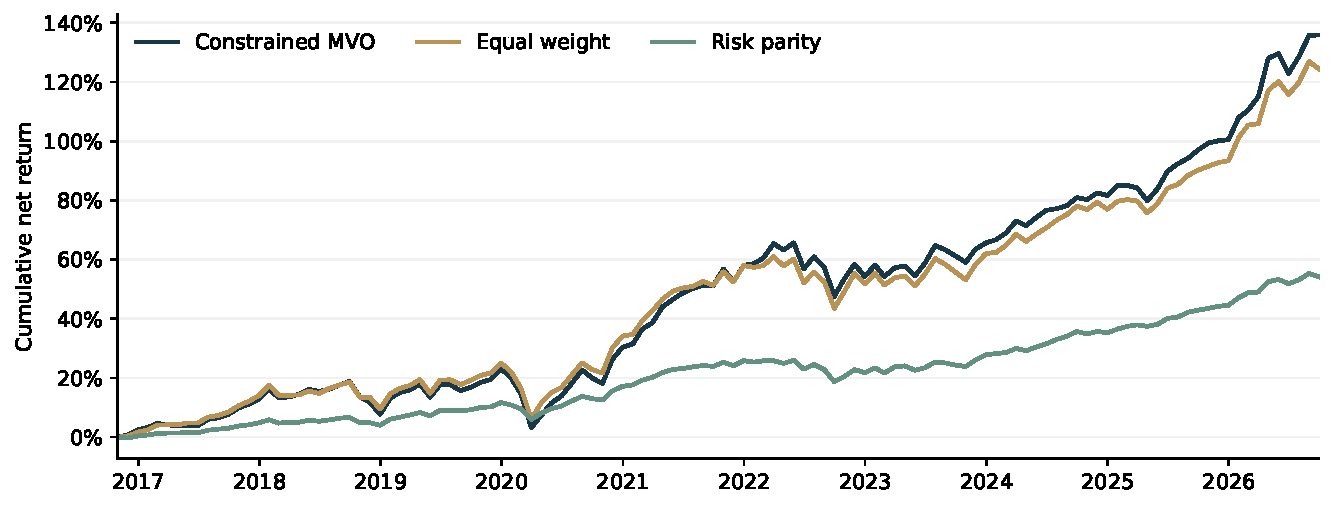
\includegraphics[width=\linewidth]{cumulative-returns.pdf}
\caption{Cumulative net returns of the fixed target allocations. Weights were selected using information through September 2026; this is a retrospective illustration.}
\end{figure}

\clearpage
\section{Backtest Protocol}\label{sec:cp3}
\subsection{Design and validation}
The main test holds the proposed target weights fixed and restores them monthly over November 2016-September 2026 (119 monthly returns). The allocation uses October 2021-September 2026 for its numerical fit. Historical results were also reviewed while choosing ETFs, limits and methods, so there is no genuinely untouched historical holdout. Separate checks fitted different weights before November 2016 or November 2021 and evaluated them on subsequent returns. These are conditional historical validation checks, not tests of the exact proposed allocation. Earlier quarterly re-optimization tests are separate research and are not the main backtest.

\subsection{Variations tried}
Earlier research included 17 method labels, six equity-sleeve variants, four peer-ETF variants, eight team-draft variants, 18 diversification subsets, eight walk-forward rules, three no-XLE variants and six alternative risk-parity universes. It also included 255-subset screens, different fitting windows and cost assumptions; one three-variant 36-month test failed. The fixed-SAA comparison evaluates three rules across the retrospective test and two historical-fit checks (nine rule/protocol evaluations). Subsequent robustness work examines 108 constraint settings, 32 return-input scenarios, 33 volatility ceilings, three historical stress periods and three hypothetical shocks. These are overlapping study counts, not independent strategy trials, and the later diagnostics did not change the selected allocation. A complete count of any additional tests by other teammates is unavailable. The reproducible retained studies are in supplementary\_studies.ipynb and studies/; the earlier research list describes explored alternatives, not additional submitted code files.

\subsection{Risk and performance}
The main MVO results are 8.60\% realized volatility, -16.19\% maximum month-end drawdown, 3.68\% historical monthly 95\% VaR and a Sharpe of 0.768. For month-end wealth $W_t$, including initial capital $W_0$, we use
\[
\mathrm{MDD}=\min_{1\leq t\leq N}\left(\frac{W_t}{\max_{0\leq s\leq t}W_s}-1\right)
\qquad
\mathrm{VaR}^{\mathrm{hist}}_{0.95}=-Q_{0.05}(r^{\mathrm{net}})
\]
The quantile uses linear interpolation. Intramonth losses are not measured.

\subsection{Discounted Sharpe}
We apply a 50\% judgmental haircut to the retrospective Sharpe:
\[
\mathrm{SR}_{\mathrm{discounted}}=0.5\,\mathrm{SR}_{\mathrm{historical}}
\approx0.5\times0.768=0.384
\] Many alternatives were inspected, the final fitting window overlaps the evaluation period, and expected returns are uncertain. The discount is a conservative reporting assumption, not a statistically estimated Deflated Sharpe Ratio, a confidence bound or a forecast of the challenge Sharpe.


\clearpage
\section{Code: Risk Budget and Evaluation}\label{sec:code}
\subsection{Data and inputs}
We use the supplied Bloomberg USD month-end price export as the ETF return input and independent FRED DGS1MO yields for the risk-free proxy. The export contains 180 prices per ETF, October 2011--September 2026, giving 179 monthly returns. The SPY download formula confirms dividend and split adjustments; the other six ETF columns are saved values, so their original adjustment settings are not preserved in the export. For ETF $i$, the monthly return is
\[
r_{i,t}=\frac{P^{\mathrm{adj}}_{i,t}}{P^{\mathrm{adj}}_{i,t-1}}-1
\]
where $P^{\mathrm{adj}}_{i,t}$ is the adjusted month-end price input. The fitting window contains 60 returns, October 2021--September 2026; no missing months were filled for the selected ETFs. We annualize the monthly arithmetic means and sample covariance matrix as
\[
\widehat\mu_{\mathrm{ann}}=12\bar r\qquad
\widehat\Sigma_{\mathrm{ann}}=12\widehat\Sigma_{\mathrm{month}}
\]
These historical means are uncertain estimates of expected returns. Tables below show all seven eligible ETFs; VWO received zero weight, while XLE was excluded.

Annual input estimates: historical arithmetic mean and sample volatility, October 2021--September 2026. Percentages are rounded for display; calculations use full precision.


\begin{center}\footnotesize
\begin{tabular}{@{}lrr@{}}\toprule
ETF & Annual mean input & Annual volatility\\
\midrule
SPY & 14.11\% & 15.67\%\\
VWO & 7.45\% & 14.74\%\\
EEMV & 6.65\% & 11.95\%\\
DBC & 13.71\% & 17.28\%\\
SCHD & 10.19\% & 15.10\%\\
VGSH & 1.83\% & 2.08\%\\
STIP & 2.88\% & 2.83\%\\
\bottomrule\end{tabular}\end{center}

Correlations of the same monthly USD returns. Values are rounded to three decimals.


\begin{center}\footnotesize
\begin{tabular}{@{}lrrrrrrr@{}}\toprule
ETF & SPY & VWO & EEMV & DBC & SCHD & VGSH & STIP\\
\midrule
SPY & 1.000 & 0.635 & 0.666 & 0.119 & 0.708 & 0.377 & 0.565\\
VWO & 0.635 & 1.000 & 0.880 & 0.142 & 0.529 & 0.514 & 0.451\\
EEMV & 0.666 & 0.880 & 1.000 & 0.039 & 0.516 & 0.527 & 0.503\\
DBC & 0.119 & 0.142 & 0.039 & 1.000 & 0.370 & -0.173 & 0.170\\
SCHD & 0.708 & 0.529 & 0.516 & 0.370 & 1.000 & 0.358 & 0.549\\
VGSH & 0.377 & 0.514 & 0.527 & -0.173 & 0.358 & 1.000 & 0.760\\
STIP & 0.565 & 0.451 & 0.503 & 0.170 & 0.549 & 0.760 & 1.000\\
\bottomrule\end{tabular}\end{center}

\subsection{Optimization}
We estimate mean returns and covariances from the same 60 monthly observations, then choose every eligible weight jointly. At a fixed 8\% estimated volatility and a common risk-free rate, maximizing estimated return also maximizes estimated Sharpe:
\[
\max_w\;w^\top\widehat\mu_{\mathrm{ann}}
\qquad\text{subject to}\qquad
\sum_i w_i=1\quad w_i\geq0\quad
\sqrt{w^\top\widehat\Sigma_{\mathrm{ann}}w}=0.08
\] The additional capital floors and risk-share caps are listed in Checkpoint 1. SciPy’s SLSQP solver uses analytic derivatives and 200 starting points across two random seeds; repeated solutions support numerical stability but do not prove a global optimum. The rounded selected weights give 7.9996\% estimated annual volatility. SPY and DBC reach approximately 40\% risk each, and VGSH reaches its 5\% capital floor. The other weights jointly balance return, covariance and the remaining limits. Excel contains the corresponding calculations; the exported recommendation was generated in Python.

\subsection{Files submitted separately}
{\raggedright
round1\_analysis.ipynb contains the data preparation, return and covariance estimates, constrained optimization, risk contributions, comparisons with equal weight and risk parity, fixed-weight monthly-rebalanced backtest, and opening share quantities. supplementary\_studies.ipynb contains the constraint and input sensitivity checks, alternative historical fitting windows, trading-cost sensitivity, frontier, stress tests, expected shortfall, rolling volatility and return attribution. data/ contains the Bloomberg workbook, monthly Bloomberg and earlier Yahoo price series, FRED yields and opening positions. results/ contains the main tables and report charts; studies/ contains supporting tables and charts. requirements.txt lists the Python packages. The saved notebooks show the steps, formulas and outputs and can be rerun from the round-1 folder.\par}

\subsection{Performance calculations}
The gross monthly return and the weights after price drift are
\[
g_t=\sum_i w_i r_{i,t}\qquad\widetilde w_{i,t}=\frac{w_i(1+r_{i,t})}{1+g_t}
\]
At the next rebalance, the traded fraction is the sum of absolute differences between the target and drifted weights, counting purchases and sales without dividing by two. Initial investment has $T_1=1$. Net monthly returns include the charge at the start of the month:
\[
T_{t+1}=\sum_i\left|w_i-\widetilde w_{i,t}\right|\qquad r^{\mathrm{net}}_t=(1-0.001T_t)(1+g_t)-1
\]
The 10 bp charge is a modelling assumption, not a quoted execution cost. Fund expenses are reflected in fund prices and are not deducted again.

\subsection{Sharpe and risk-free rate}
Let $y_{t^-}$ be the last available FRED DGS1MO percentage yield strictly before month $t$, and $d_t$ the number of calendar days in that month. The risk-free proxy is
\[
r_{f,t}=\frac{y_{t^-}}{100}\frac{d_t}{365}
\]
This approximates interest accrual; it is not a traded T-bill total-return index. Using $N$ net monthly returns and sample standard deviation $s$, we calculate
\[
\mathrm{SR}_{\mathrm{ann}}=\sqrt{12}\frac{\overline{r^{\mathrm{net}}-r_f}}{s(r^{\mathrm{net}})}
\qquad
\sigma_{\mathrm{ann}}=\sqrt{12}\,s(r^{\mathrm{net}})
\]
\[
\mathrm{CAGR}=\left[\prod_{t=1}^{N}(1+r^{\mathrm{net}}_t)\right]^{12/N}-1
\]


\clearpage
\section{Portfolio Description}\label{sec:portfolio}


\subsection{Portfolio implementation}
Bloomberg entry date: 16 October 2026. Price date: the close of Friday, 16 October 2026. Initial capital: \$100{,}000{,}000.00.
For capital $C$, target weight $w_i$ and closing price $P_i$, the unrounded share quantity is
\[
q_i^*=\frac{w_i C}{P_i}
\]
We then converted these quantities to whole shares. Small round-ups used the remaining cash while keeping the portfolio within budget. The final STIP quantity includes four additional shares. The table shows the selected target weights rounded to two decimals; actual capital weights differ only slightly because shares are indivisible.

\begin{table}[H]
\centering
\small
\renewcommand{\arraystretch}{1.3}
\arrayrulecolor{line}
\begin{tabularx}{\textwidth}{@{}>{\raggedright\arraybackslash}X l c r r c@{}}
\toprule
\hd{ETF name} & \hd{Bloomberg ID} & \hd{Curr.} & \hd{\# shares} & \hd{Weight} & \hd{Price date}\\
\midrule
State Street SPDR S\&P 500 ETF Trust          & SPY US & USD & 34,169 & 26.08\% & 16/10/2026\\
iShares MSCI Emerging Markets Min Vol Factor ETF & EEMV US & USD & 133,610 &  9.66\% & 16/10/2026\\
Invesco DB Commodity Index Tracking Fund      & DBC US & USD & 798,756 & 26.95\% & 16/10/2026\\
Vanguard Short-Term Treasury Index Fund ETF   & VGSH US & USD & 86,671 &  5.00\% & 16/10/2026\\
Schwab U.S. Dividend Equity ETF               & SCHD US & USD & 95,488 &  3.28\% & 16/10/2026\\
iShares 0--5 Year TIPS Bond ETF               & STIP US & USD & 288,630 & 29.03\% & 16/10/2026\\
\midrule
\hd{Total} & & & & \hd{100.00\%} & \\
\bottomrule
\end{tabularx}
\caption{Opening positions at the supplied 16 October 2026 closing prices. All Bloomberg identifiers use the Equity market sector (for example, SPY US Equity). Weights are targets rounded to two decimals.}
\label{tab:portfolio}
\end{table}

Opening market value: \$99,999,987.88. Remaining cash: \$12.12. Total: \$100,000,000.00. Closing prices (USD, 16 October 2026): SPY 763.25; EEMV 72.30; DBC 33.74; VGSH 57.69; SCHD 34.35; STIP 100.58. These share quantities and prices are the opening implementation; the historical backtest uses the target weights and its stated trading-cost assumption.

\subsection{The six ETFs}
All six funds are passive and track a public index. The table gives the key facts; the notes below
describe what each fund holds.

\begin{table}[H]
\centering
\small
\renewcommand{\arraystretch}{1.25}
\arrayrulecolor{line}
\begin{tabularx}{\textwidth}{@{}l l >{\raggedright\arraybackslash}X l r@{}}
\toprule
\hd{ETF} & \hd{Launch} & \hd{Index tracked} & \hd{Holdings} & \hd{Expense ratio}\\
\midrule
SPY  & 22 Jan 1993 & S\&P 500 & about 500 stocks & 0.0945\%\\
EEMV & 18 Oct 2011 & MSCI Emerging Markets Minimum Volatility & 297 stocks & 0.25\%\\
DBC  & 3 Feb 2006  & DBIQ Optimum Yield Diversified Commodity Index ER & Diversified futures & 0.84\% net\\
VGSH & 19 Nov 2009 & Bloomberg US Treasury 1--3 Year & 90--95 Treasury notes & 0.03\%\\
SCHD & 20 Oct 2011 & Dow Jones U.S. Dividend 100 & about 100 stocks & 0.06\%\\
STIP & 1 Dec 2010  & ICE U.S. Treasury 0--5 Year Inflation Linked Bond & 24 holdings & 0.03\%\\
\bottomrule
\end{tabularx}
\caption{Key facts of the six ETFs (fund fact sheets, October 2026).}
\label{tab:etfs}
\end{table}

\subsubsection*{SPY \,$\cdot$\, State Street SPDR S\&P 500 ETF Trust}
The first ETF ever listed in the US, structured as a unit investment trust. It matches the price and yield of the
S\&P 500, a float-adjusted, market-cap-weighted index of large US companies across all eleven GICS sectors.
It is tilted towards Information Technology (38.38\% on 15 Oct 2026), with NVIDIA, Apple and Microsoft as the largest
positions. It pays dividends quarterly, with a yield of about 1\%.
\href{https://www.ssga.com/us/en/intermediary/etfs/state-street-spdr-sp-500-etf-trust-spy}{\textcolor{gold}{Source}}

\subsubsection*{EEMV \,$\cdot$\, iShares MSCI Emerging Markets Min Vol Factor ETF}
It holds emerging-market stocks with lower volatility than the broader MSCI Emerging Markets Index, keeping
equity exposure at lower risk (3-year beta of 0.62). The portfolio is concentrated in Taiwan (23.49\%),
China (19.58\%), India (16.50\%) and South Korea (13.98\%), and in Information Technology
(34.80\% on 15 Oct 2026) and Financials (21.25\%). It pays income semi-annually.
\href{https://www.ishares.com/us/products/239641/ishares-msci-emerging-markets-minimum-volatility-etf}{\textcolor{gold}{Source}}

\subsubsection*{DBC \,$\cdot$\, Invesco DB Commodity Index Tracking Fund}
A commodity pool providing diversified exposure to energy, precious metals, industrial metals and agriculture,
accessed through futures rather than physical goods. The index is designed to maximise roll benefits in
backwardated markets and limit roll losses in contango. Its return comes from price changes, roll yield and
the interest on its Treasury collateral. Invesco updated the index methodology in November 2025, including broader eligibility and concentration limits. The listed total and net expense ratios are 0.89\% and 0.84\%.
\href{https://www.invesco.com/content/dam/invesco/us/en/product-documents/etf/fact-sheet/dbc-invesco-db-commodity-index-tracking-fund-fact-sheet.pdf}{\textcolor{gold}{Source}}

\subsubsection*{VGSH \,$\cdot$\, Vanguard Short-Term Treasury ETF}
It holds US Treasury notes with 1 to 3 years to maturity, excluding TIPS, almost entirely in government
bonds (about 99.7\%). It samples the index instead of holding every bond. Its short duration makes it
little sensitive to interest rates, and it pays income monthly.
\href{https://investor.vanguard.com/investment-products/etfs/profile/vgsh}{\textcolor{gold}{Source}}

\subsubsection*{SCHD \,$\cdot$\, Schwab U.S. Dividend Equity ETF}
It selects about 100 US large-cap stocks for the quality and sustainability of their dividends, judged on
financial ratios relative to peers. It is tilted towards Health Care, Consumer Staples and Energy; top holdings
include Texas Instruments, Procter \& Gamble, Chevron and Coca-Cola. It pays dividends quarterly, with a
yield of about 3.2\%.
\href{https://www.schwabassetmanagement.com/products/schd}{\textcolor{gold}{Source}}

\subsubsection*{STIP \,$\cdot$\, iShares 0--5 Year TIPS Bond ETF}
It held 24 positions on 15 October 2026, with 94.75\% in Treasuries (reported in the AA category) and 5.25\% in cash and/or derivatives. Its Treasury Inflation-Protected Securities have less than five years to maturity. The principal adjusts with inflation, so it hedges rising prices while keeping interest-rate risk low
(effective duration 2.25 years on 15 October 2026). It pays income monthly.
\href{https://www.blackrock.com/us/individual/products/239450/ishares-0-5-year-tips-bond-etf}{\textcolor{gold}{Source}}

% ---------- allocation charts ----------
\subsection{Allocation charts}
\begin{figure}[H]\centering
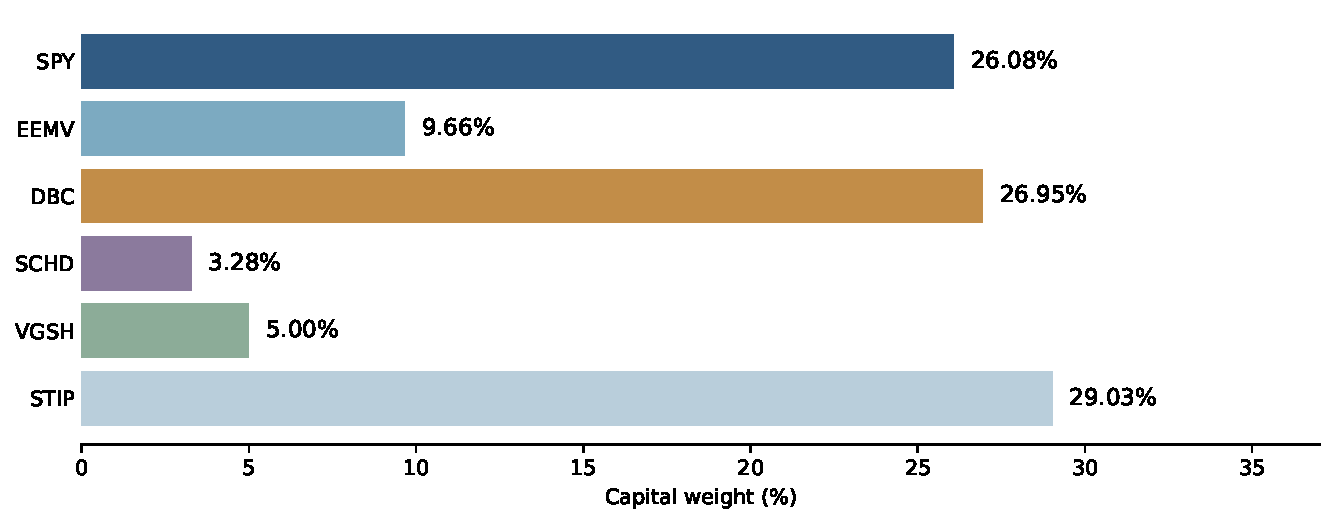
\includegraphics[width=.9\linewidth]{allocation.pdf}
\caption{Final capital weights by ETF.}\end{figure}
\begin{figure}[H]\centering
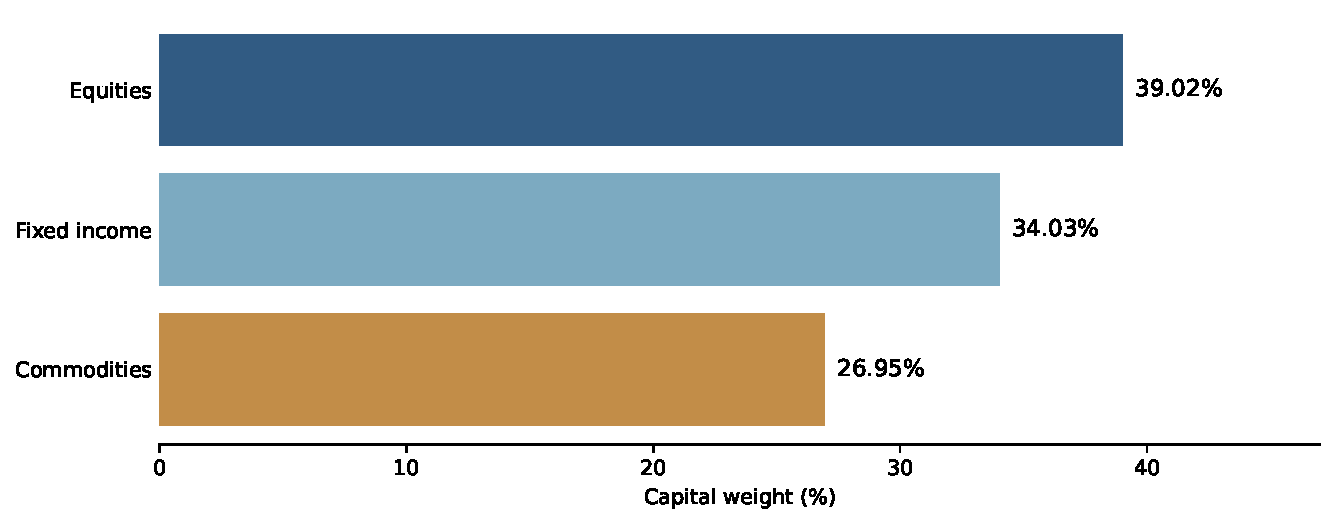
\includegraphics[width=.9\linewidth]{asset-classes.pdf}
\caption{Final allocation by asset class.}\end{figure}

\clearpage
\appendix\section{Supplementary Analysis}\label{sec:supplementary}
These studies examine how the allocation changes when we alter the limits or return estimates, and how it behaves in stressed markets. They did not change the opening positions. As they use history already reviewed during portfolio selection, they do not provide an untouched validation sample.

\subsection{Changing the risk cap}
Lowering the maximum ETF risk share from 40\% to 37.5\% reallocates 3.64\% of capital; raising it to 42.5\% reallocates 3.83\%. Wider changes to 35\% and 45\% reallocate 7.10\% and 11.76\%. For alternative and baseline weights, the fraction of capital reallocated is
\[
A=\frac12\sum_i\left|w_i^{\mathrm{alternative}}-w_i^{\mathrm{baseline}}\right|
\]
The 40\% cap is our chosen concentration limit; these tests do not establish it as an optimal value.

\subsection{Changing the return estimates}
Adding one percentage point to VGSH's estimated annual return reallocates 28.84\% of capital, mainly between the two bond funds. Evaluated with the original return estimates, this alternative's expected return is only 6.38 basis points below the baseline. The optimizer can therefore produce quite different weights with similar objective values. The precise weights depend heavily on the return estimates.

\subsection{Risk over time}
Annualized volatility in rolling 12-month windows ranges from 3.04\% to 16.51\%. Our initial 8\% estimate does not keep every subsequent window inside 7--9\%. The challenge band applies to the estimated SAA risk.

\subsection{Stress tests}
Applying the selected weights to historical stress periods gives gross returns of -9.35\% in 2018 Q4, -13.82\% in February--March 2020 and -2.35\% over 2022. These periods differ in length and exclude trading costs, so they should not be compared directly with one-month VaR. Hypothetical growth, commodity-reversal and inflation/rate shocks give -11.89\%, -12.05\% and -2.49\%, respectively. The ETF-level shocks are specified in supplementary\_studies.ipynb, without an assigned probability or time horizon.

\subsection{Losses in the worst months}
Net historical one-month 95\% expected shortfall is 5.67\%, equivalent to USD 5.67 million on initial capital, compared with 3.68\% historical VaR. Expected shortfall averages losses in the worst 5\% of months, with fractional weighting at the cutoff. Both estimates use only 119 monthly observations.

\subsection{The return--risk trade-off}
The frontier plots historical arithmetic mean return against estimated volatility while retaining our capital floors and concentration caps. Its shape depends on the chosen historical inputs; it does not predict future returns.

\subsection{Where the returns came from}
Linked return attribution assigns about USD 57.61 million to SPY and USD 49.13 million to DBC out of the backtest's USD 135.90 million net profit. The portfolio's historical gains were concentrated in these two funds, which also account for most of its estimated risk.

\begin{figure}[H]\centering
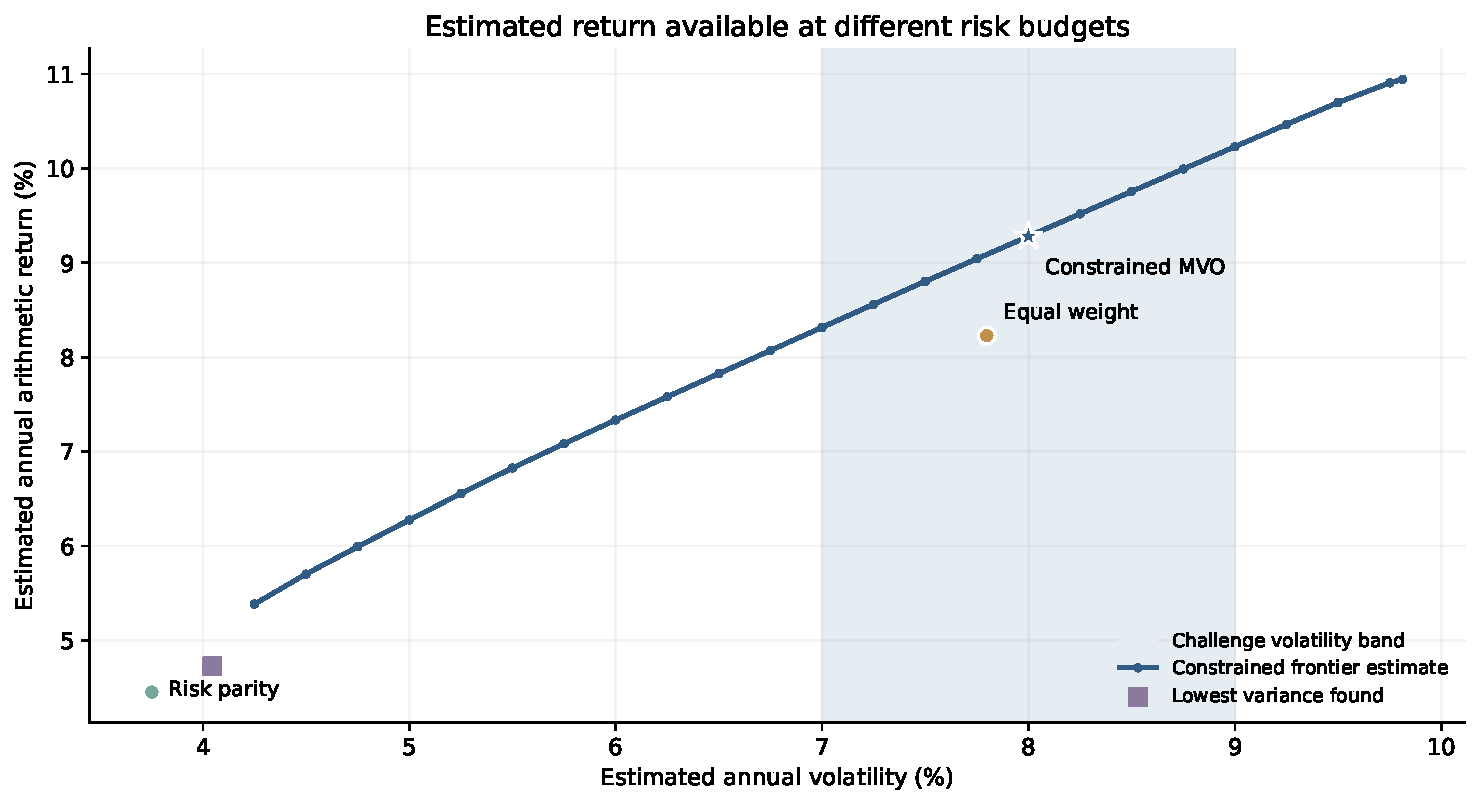
\includegraphics[width=\linewidth]{efficient-frontier.pdf}
\caption{Estimated return--risk frontier, conditional on historical mean returns and the capital floors and concentration caps. The curve varies the volatility ceiling; the challenge band is 7--9\%.}\end{figure}
\begin{figure}[H]\centering
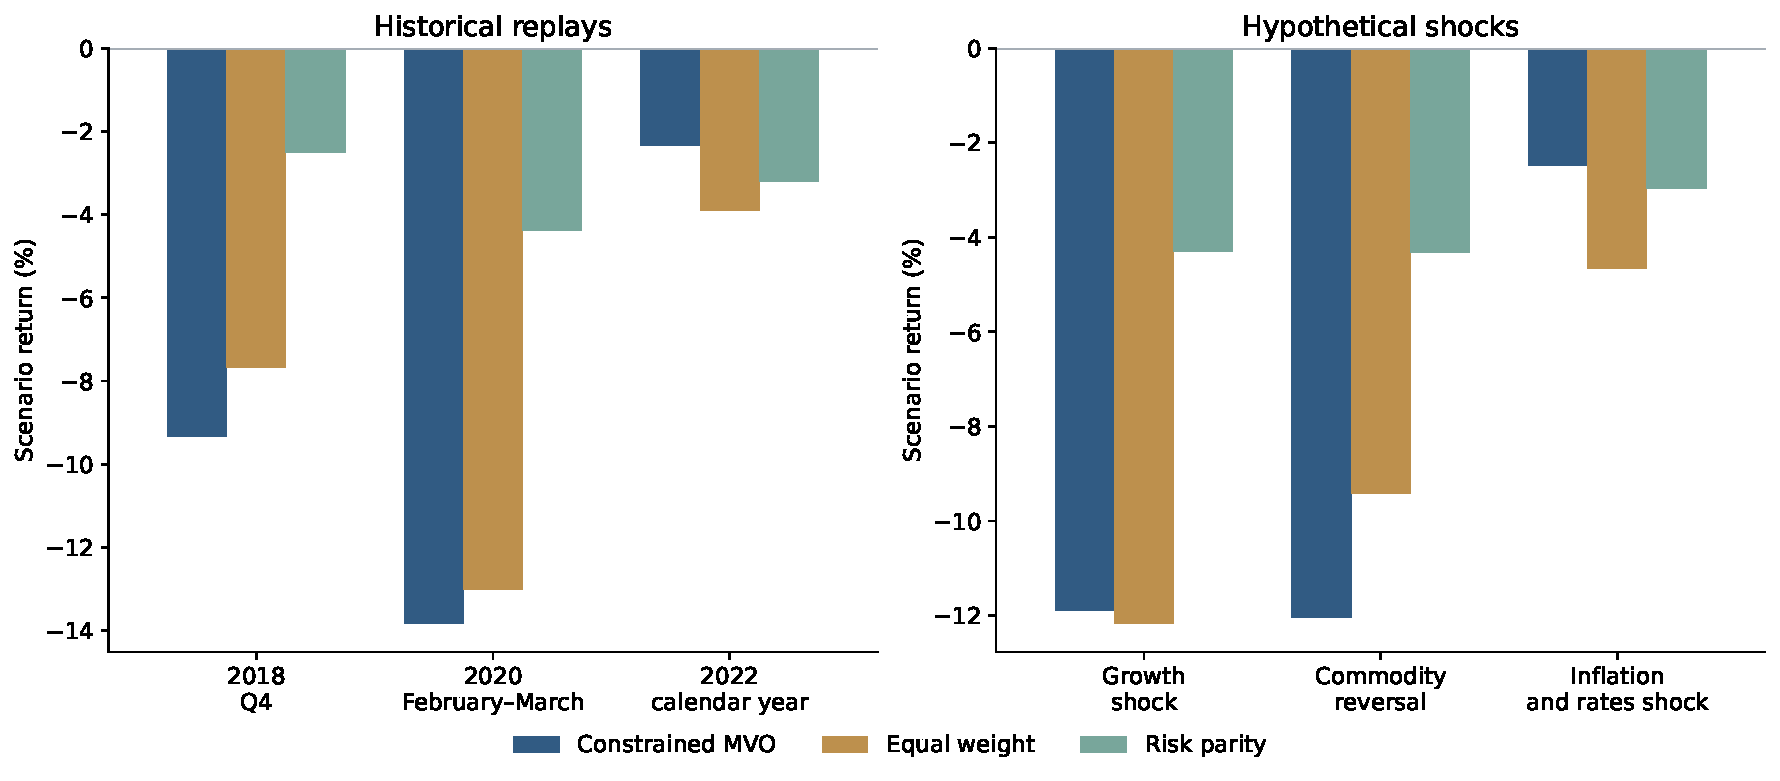
\includegraphics[width=\linewidth]{stress-comparison.pdf}
\caption{Historical and hypothetical scenario returns. Historical periods differ in length; hypothetical shocks have no assigned probability or horizon. Scenario assumptions and calculations are in the supplementary notebook.}\end{figure}

\end{document}